\chapter{Estimating the bank erosion} \label{Chp:BankErosion}

\dfastbe is intended to be a tool to help to estimate the potential for bank erosion and not to accurately predict the actual bank erosion.
Two bank erosion mechanisms are included: erosion due to ship waves and erosion due to currents.

These two mechanisms are discussed in more detailed in the first two sections of this chapter, followed by a brief description of the total bank line shift and the algorithm for moving the bank lines for a constant discharge in \autoref{Sec4.3}.
Subsequently, \autoref{Sec4.4} describes the way in which the total potential bank erosion volume is determined.
\autoref{Sec4.5} explains how to deal with variations in the discharge, and \autoref{Sec4.6} introduces the equilibrium bank erosion concept and the corresponding volume of eroded material.
Finally, a number of limitations of the software are listed in \autoref{Sec4.7}.

\section{List of symbols} \label{Sec:SymbolList}

\begin{symbollist}
\item[$C$] Ch\'ezy coefficient representing hydraulic roughness \unitbrackets{m\textsuperscript{1/2}/s}
\item[$c_E$] strength coefficient of the bank material \unitbrackets{m\textsuperscript{-1}s\textsuperscript{-1}}
\item[$E$] erosion coefficient \unitbrackets{m/s}
\item[$g$] gravitational acceleration, i.e. 9.81 \unitbrackets{m/s\textsuperscript{2}}
\item[$H$] wave height at the bank \unitbrackets{m}
\item[$H_0$] initial wave height at the toe of the foreshore \unitbrackets{m}
\item[$h$] water depth \unitbrackets{m}
\item[$h_s$] bank height above the top level $z_\text{up}$ of the range of influence for equilibrium erosion \unitbrackets{m}
\item[$h_t$] elevation range directly affected by equilibrium erosion: $z_\text{up} - z_\text{do}$ \unitbrackets{m}
\item[$N$] number of empty ships per year \unitbrackets{1/year}
\item[$N_r$] number of reed stems per square meter \unitbrackets{m\textsuperscript{-2}}
\item[$N_\text{sec}$] number of seconds in a year: 31536000 \unitbrackets{-}
\item[$n$] number of waves per ship \unitbrackets{-}
\item[$n_Q$] number of discharge levels included \unitbrackets{-}
\item[$p(Q_i)$] yearly probability of discharge $Q_i$ \unitbrackets{-}
\item[$s$] distance from ship to shore \unitbrackets{m}
\item[$s_0$] distance from ship at which the ship waves have reduced to zero \unitbrackets{m}
\item[$s_1$] distance from ship at which the ship waves start to reduce \unitbrackets{m}
\item[$t$] time \unitbrackets{s}
\item[$T$] period of the ship waves \unitbrackets{s}
\item[$T_s$] draught of the ship \unitbrackets{m}
\item[$t_\text{eros}$] bank erosion analysis period \unitbrackets{s}
\item[$u_b$] flow velocity along the bank line \unitbrackets{m/s}
\item[$u_c$] critical flow velocity for erosion \unitbrackets{m/s}
\item[$v_s$] ship velocity \unitbrackets{m/s}
\item[$V_\text{eq}$] eroded sediment volume until equilibrium \unitbrackets{m\textsuperscript{3}}
\item[$V_\text{erosion}$] eroded sediment volume over a period $t_\text{eros}$ \unitbrackets{m\textsuperscript{3}}
\item[$y$] width of the bank area \unitbrackets{m}
\item[$z_\text{bank}$] level of the top of the bank \unitbrackets{m}
\item[$z_\text{do}$] bottom level of the range of influence for equilibrium erosion \unitbrackets{m}
\item[$z_\text{prot}$] top level of the bank protection \unitbrackets{m}
\item[$z_\text{up}$] top level of the range of influence for equilibrium erosion \unitbrackets{m}
\item[$z_w$] water level \unitbrackets{m}
\item[$\alpha$] coefficient in the relation between critical shear stress for erosion and the erosion coefficient \unitbrackets{m\textsuperscript{-3/2} kg\textsuperscript{1/2}}
\item[$\alpha_1$] ship dependent wave generation coefficient \unitbrackets{-}
\item[$\delta h_\text{above}$] bank erosion distance above the water surface \unitbrackets{m}
\item[$\delta h_\text{below}$] bank erosion distance below the water surface \unitbrackets{m}
\item[$\Delta n(Q_i)$] total shift of the bank line at discharge $Q_i$ \unitbrackets{m}
\item[$\Delta n_\text{eq}$] erosion distance until equilibrium \unitbrackets{m}
\item[$\Delta n_\text{flow}$] bank line shift due to currents over a period $t_\text{eros}$ \unitbrackets{m}
\item[$\Delta n_\text{flow}(Q_i)$] shift of the bank line due to currents at discharge $Q_i$ \unitbrackets{m}
\item[$\Delta n_\text{tot}$]  total shift of the bank line \unitbrackets{m}
\item[$\Delta n_\text{wave}$] shift of bank line due to ship waves \unitbrackets{m}
\item[$\Delta n_\text{wave}(Q_i)$] shift of the bank line due to ship waves at discharge $Q_i$ \unitbrackets{m}
\item[$\mu$] wave damping parameter \unitbrackets{m\textsuperscript{-1}}
\item[$\mu_\text{fs}$] wave damping due to sloping foreshore \unitbrackets{m\textsuperscript{-1}}
\item[$\mu_r$] wave damping due to reed \unitbrackets{m\textsuperscript{-1}}
\item[$\mu_\text{tot}$] total wave damping parameter \unitbrackets{m\textsuperscript{-1}}
\item[$\tau_c$] critical shear stress for erosion of bank material \unitbrackets{Pa}
\end{symbollist}

\section{Determining potential erosion by ship waves} \label{Sec4.1}

Ship waves are one of the most important causes of bank erosion \citep{Verheij00} and they are therefore included as the first bank erosion mechanism in the \dfastbe.
The bank erosion formula due to ship waves has been copied from the BEM module (\citet{Verheij00}, \citet{StolkerV01b}) and the quantities are defined by \autoref{Fig4.1}.

\begin{figure}[!h]
\center
\resizebox{10cm}{!}{
   \input{figures/crosssec.pdf_tex}
}
\caption{Graphical definition of quantities}
\label{Fig4.1}
\end{figure}

Based on large scale Delta flume experiments, in which slopes of various materials were subject to perpendicular waves, it has been derived that the erosion rate increases quadratically as function of the wave height at the bank
%
\begin{equation}
\diff{y}{t} = c_E H^2
\label{Eq1.1}
\end{equation}
%
where
%
\begin{symbollist}
\item[$y$] width of the bank area \unitbrackets{m}
\item[$c_E$] strength coefficient of the bank material \unitbrackets{m\textsuperscript{-1}s\textsuperscript{-1}}
\item[$H$] wave height at the bank \unitbrackets{m}
\end{symbollist}

The value $c_E$ representing the bank strength depends on the composition of the bank and can thus vary spatially.
The $c_E$ values for the five supported bank compositions classes are given in \autoref{Tab4.1}; for additional values see \autoref{bankcomp}.
For the computations, the user specifies the bank composition class in a simple text file along the analyzed reach.
%
\clearpage
\begin{table}[!h]
	\center
	\begin{tabular}{llll}
		Class & Bank composition & $c_E$ \unitbrackets{m\textsuperscript{-1} s\textsuperscript{-1}} & $\tau_c$ \unitbrackets{Pa} \\ \hline
		0 & Protected bank & 0 & $\infty$ \\
		1 & Vegetated bank & 0.02 10\textsuperscript{-4} & 95 \\
		2 & Good quality clay & 0.6 10\textsuperscript{-4} & 3 \\
		3 & Medium to poor quality clay & 2 10\textsuperscript{-4} & 0.95 \\
		4 & Sand & 12.5 10\textsuperscript{-4} & 0.15 \\ \hline
	\end{tabular}
	\caption{Bank composition classes supported by \dfastbe}
	\label{Tab4.1}
\end{table}
%
Generally, it's assumed that the wave height decreases negative exponentially as function of the width of the bank area
%
\begin{equation}
H = H_0 e^{-\mu y}
\label{Eq1.2}
\end{equation}
%
where
%
\begin{symbollist}
\item[$H_0$] initial wave height at the toe of the foreshore \unitbrackets{m} (see \autoref{Sec:shipwaves})
\item[$\mu$] wave damping parameter \unitbrackets{m\textsuperscript{-1}}
\end{symbollist}
%
Substitution of \autoref{Eq1.2} in \autoref{Eq1.1} results in a differential equation with general solution
%
\begin{equation}
\Delta n_\text{wave} = \frac{1}{2 \mu} \ln ( 2 \mu c_E H_0^2 t + 1 )
\end{equation}
%
where
%
\begin{symbollist}
\item[$\Delta n_\text{wave}$] shift of bank line due to ship waves \unitbrackets{m}
\item[$t$] time \unitbrackets{s}
\end{symbollist}
%
This equation can be used for waves due to both wind and ships.
Since $\mu c_E H_0^2$ is typically small, the equation implemented in \dfastbe is therefore linearized to
%
\begin{equation}
\Delta n_\text{wave} = c_E H_0^2 t
\end{equation}
%
In the latter case the effective time $t$ can be expressed as
%
\begin{equation}
t = T N n t_\text{eros} = 0.51 \frac{v_s}{g} N n t_\text{eros}
\end{equation}
%
where
%
\begin{symbollist}
\item[$T$] period of the ship waves \unitbrackets{s}
\item[$N$] number of empty ships per year \unitbrackets{1/year}
\item[$n$] number of waves per ship \unitbrackets{-}
\item[$v_s$] ship velocity \unitbrackets{m/s}
\item[$g$] gravitational acceleration, i.e. 9.81 \unitbrackets{m/s\textsuperscript{2}}
\item[$t_\text{eros}$] bank erosion analysis period \unitbrackets{s}
\end{symbollist}
%
The value of the initial wave height $H_0$ at the toe of the foreshore can be computed using equations such as included in DIPRO based on the characteristic vessel type, its sailing speed and draught, the distance between the navigation channel and the bank and the water depth (see \autoref{Sec:shipwaves}).

The parameter $\mu$ can be used to account for not only the effect of the shape of the foreshore on wave damping, but also for the wave damping effect of foreshore constructions, vegetation, and deposits of bank material.
The bank erosion module includes the effect of the slope of the foreshore and the vegetation on the wave damping.
The wave damping due to a gently sloping foreshore is given by \citet{Verheij00} as
%
\begin{equation}
\mu_\text{fs} = \frac{\tan(\alpha)}{H_0}
\end{equation}
%
where $\tan \alpha = \frac{1}{n}$ for a foreshore with 1:$n$ slope (see also \autoref{Fig4.1}).
For an initial wave height $H_0 = 0.4$ a slope between 1:100 and 1:20 results in values for $\mu_\text{fs}$ between 0.025 and 0.125.
\autoref{Fig4.2} shows an example of the influence of the wave damping parameter $\mu_\text{fs}$ on the bank erosion due to waves.

\begin{figure}[!hb]
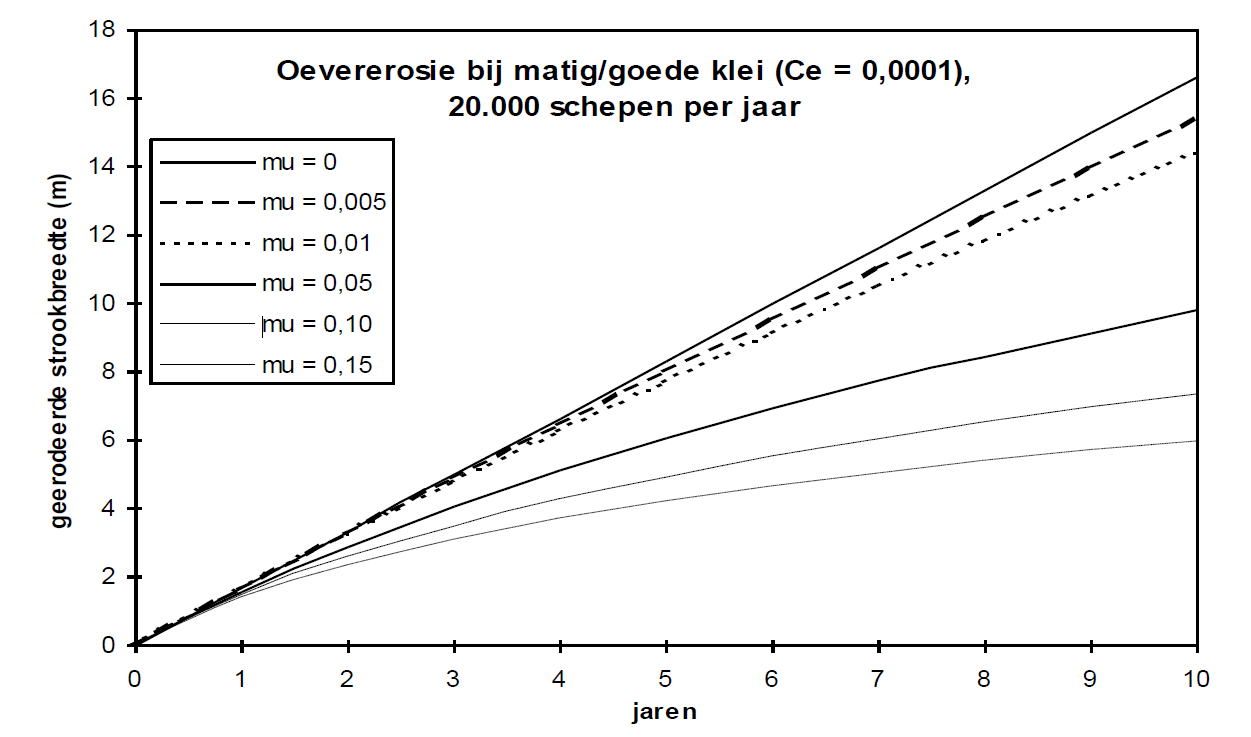
\includegraphics[width=\textwidth]{figures/Fig4-2.png}
\caption{Example of bank erosion due to waves for average to good clay with a bankstrenght coefficient ($c_E$ = 0.0001). An increase in the parameter $\mu_\text{fs}$ accounts for an increased effect of the shape of the foreshore on wave damping}
\label{Fig4.2}
\end{figure}

Besides wave damping due to foreshore slope, the incoming waves can also be dampened by the presence of vegetation.
The following equation can be used to estimate the wave damping due to reed
%
\begin{equation}
\mu_r = 8.5 \cdot 10^{-4} N_r^{0.8}
\end{equation}
%
where $N_r$ is the reed stem density (number of stems per square metre).
The combined wave damping effect due to foreshore slope and reed is given by
%
\begin{equation}
\mu_\text{tot} = \mu_\text{fs} + \mu_r
\end{equation}
%
\clearpage
\section{Determining ship induced wave height at the beginning of the foreshore} \label{Sec:shipwaves}

To determine the ship induced wave height $H_0$ \unitbrackets{m} at the beginning of the foreshore, the following formula is used (source: Handleiding DIPRO, 1997)
%
\begin{equation}
H_0 = \alpha_1 h \left ( \frac{s}{h} \right )^{-1/3} \Frou^4
\end{equation}
%
with
%
\begin{symbollist}
\item[$\alpha_1$] ship dependent coefficient \unitbrackets{-}
\item[$\Frou$] Froude number ($\Frou < \text{0.8}$) \unitbrackets{-}
\item[$h$] water depth (considering a  trapezoidal profile) \unitbrackets{m}
\item[$s$] distance from ship to shore \unitbrackets{m}
\end{symbollist}
%
The Froude number, a dimensionless quantity indicating the mean flow velocity relative to the speed of free surface waves, is computed as:
%
\begin{equation}
\Frou = \frac{v_s}{\sqrt{g h}}
\end{equation}
%
with
%
\begin{symbollist}
\item[$g$] gravity acceleration 9.81 \unitbrackets{m/s\textsuperscript{2}}
\item[$v_s$] ship velocity \unitbrackets{m/s}
\end{symbollist}

The value of the Froude number is limited to 0.8 and \autoref{Tabships} shows the values used for the coefficient $\alpha_1$, with 
\begin{symbollist}
	\item[$T_s$]  the draught of the ships \unitbrackets{m}
\end{symbollist}


By using these formulas, the value of $H_0$ can be computed based on the dominant ship type, their velocity and draught, the distance between fairway and shore and the water depth.

\begin{table}[!h]
	\begin{tabular}{ll}
		Ship type & $\alpha_1$ \\ \hline
		Push barge & 0.5 \\
		RHK ship / Motorship & 0.28 $T_s^\text{1.25}$ \\
		Towboat & 1.0 \\ \hline
	\end{tabular}
	\caption{Ship-types supported by D-Fast Bank Erosion, with $T_s$ \unitbrackets{m} the draught of the ships}
	\label{Tabships}
\end{table}

\clearpage
To prevent wave load on smaller channels far from the main channel, the wave height is smoothly reduced to zero from distance $s_1$ to $s_0$ from the fairway.
This is accomplished by multiplying $H_0$ with the following function:
%
\begin{equation}
f(s) = \left \{ \begin{matrix}
1 & 0 < s < s_1 \\
\cos \left ( \frac{s - s_1}{s_0 - s_1} \pi \right ) & s_1 < s < s_0 \\
0 & s > s_0
\end{matrix} \right .
\end{equation}
%
The value for $s_0$ will be in the order of 150 - 200 m and for  the following relation is used: $s_1 = s_0 - 50$.
In \autoref{Fig5.1} the wave height $H_0$ as function of the distance from the fairway $s$ is depicted for various values of the water depth $h$ for a moter ship with a draught of 1.2 m with a relative velocity of $v_s = 6$ m/s.
The wave height is reduced to zero between $s_1 = 100$ m and $s_0 = 150$ m.

\begin{figure}[!hb]
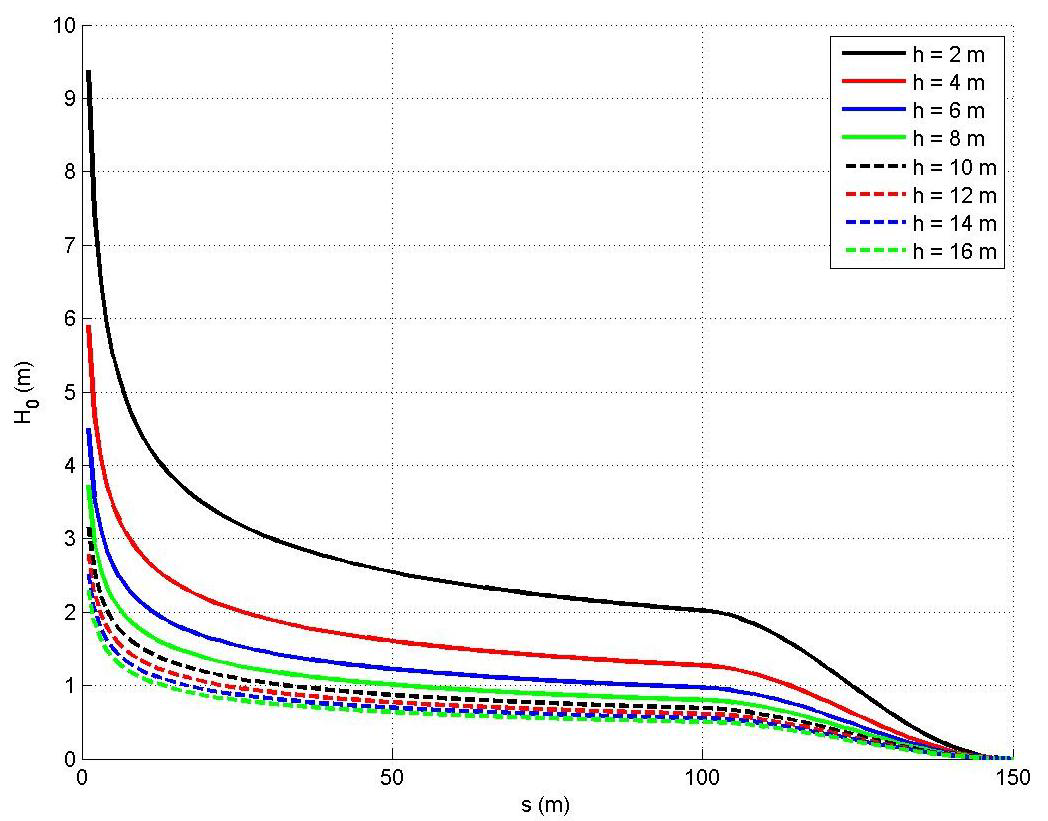
\includegraphics[width=\textwidth]{figures/Fig5-1.png}
\caption{Wave height as function from the distance from the fairway for different values of the water depth.}
\label{Fig5.1}
\end{figure}


\clearpage
\section{Determining potential erosion by currents} \label{Sec4.2}

Bank erosion can besides by ship waves also be caused by a strong current along the bank.
This mechanism is also included in the \dfastbe analysis.
For a bank line the potential for bank erosion due to currents at a certain discharge $Q$-level can be determined by the flow velocities from the model results and:
%
\begin{equation}
\Delta n_\text{flow} = E \left ( \frac{u_b^2}{u_c^2} - 1 \right ) N_\text{sec} t_\text{eros}
\end{equation}
%
where
%
\begin{symbollist}
\item[$\Delta n_\text{flow}$] bank line shift due to currents over a period $t_\text{eros}$ \unitbrackets{m}
\item[$E$] erosion coefficient \unitbrackets{m/s}
\item[$N_\text{sec}$] number of seconds in a year: 31536000 \unitbrackets{-}
\item[$u_b$] flow velocity along the bank line \unitbrackets{m/s}
\item[$u_c$] critical flow velocity for erosion \unitbrackets{m/s}
\item[$t_\text{eros}$] bank erosion analysis period \unitbrackets{s}
\end{symbollist}
%
The erosion coefficient $E$ can be determined as
%
\begin{equation}
E = \alpha \sqrt{\tau_c}
\end{equation}
%
where $\alpha$ = 2 10\textsuperscript{-7} \unitbrackets{m\textsuperscript{-3/2} kg\textsuperscript{1/2}} and $\tau_c$ \unitbrackets{N/m\textsuperscript{2}} the critical shear stress for erosion.
This value for the erosion coefficient is similar to values for erosion coefficients found in literature, e.g.~\citet{Crosato07}.

However, this relationship between the critical shear stress for erosion and the erosion coefficient is not universally valid and the user may, therefore, also specify its value directly in the input.

The critical flow velocity for erosion is related to the critical shear stress for erosion as
%
\begin{equation}
u_c = \sqrt{\frac{\tau_c}{\rho} \frac{C^2}{g}}
\end{equation}
%
where $C$ \unitbrackets{m\textsuperscript{1/2}/s} is the Ch\'ezy coefficient representing the hydraulic roughness.
The Ch\'ezy value is copied from the \dflowfm calculation.

The flow velocity along the bank line is derived from the \dflowfm flow velocities.
The value of the critical shear stress for erosion, $\tau_c$, is linked to the strength coefficient of the bank material, $c_E$ , as given by \autoref{Tab4.1} and \autoref{bankcomp}.

\section{Total bank shift} \label{Sec4.3}

The total bank line shift is determined by adding the contributions of the bank line shifts due to waves and currents
%
\begin{equation}
\Delta n = \Delta n_\text{flow} + \Delta n_\text{wave}
\end{equation}
%
The new location of the bank line is determined by locally shifting the bank line over the computed erosion distance $\Delta n$; see \autoref{Sec:BankShift} for a description how that is done.

\section{Potential bank erosion volume} \label{Sec4.4}

Besides the potential bank line shift, it's also important to know the total volume of sediment that would be associated by that potential erosion since that volume will eventually end up in the river, which may subsequently influence the bed levels and eventually trigger the need for additional dredging activities.
The potential volume of sediment released by the erosion can be estimated using
%
\begin{equation}
V_\text{erosion} = ( \delta h_\text{above} + \delta h_\text{below} ) \Delta n
\end{equation}

where 
\begin{symbollist}
	\item[$\Delta n$] total shift of the bank line [m]
	\item[$\delta h$] the area influenced by the bank erosion (above and below the water surface).
\end{symbollist}
It's assumed that the bank recedes in its entirety and that's why the area of influence above the water surface is determined by

\begin{equation}
\delta h_\text{above} = z_\text{bank} - z_w
\end{equation}
%
where
%
\begin{symbollist}
\item[$z_w$] water level \unitbrackets{m}
\item[$z_\text{bank}$] level of the top of the bank \unitbrackets{m}
\end{symbollist}
%
Note that $\delta h_\text{above} < 0$ if the bank is flooded ($z_\text{bank} < z_w$).
The extent of the area of influence \emph{below} the water surface is determined by the wave height and the level up to where the stone protection stays in place.
The following relation is used here
%
\begin{equation}
\delta h_\text{below} = \min ( z_w - z_\text{prot}, 2 H )
\end{equation}
%
where
%
\begin{symbollist}
\item[$z_w$] water level \unitbrackets{m}
\item[$z_\text{prot}$] top level of the bank protection \unitbrackets{m}
\item[$H$] wave height at the bank \unitbrackets{m}
\end{symbollist}
%
\autoref{Fig4.5} shows schematically what the eroded volume will be for different water levels.

\begin{figure}
\resizebox{\columnwidth}{!}{
   \input{figures/erodedvol.pdf_tex}
}
\caption{Eroded volume for different water levels.}
\label{Fig4.5}
\end{figure}

The retreat of the bank is completely determined by the bank erosion irrespective of the fate of the sediment -- whether the material is (temporarily) deposited on the bed in front of the bank or immediately transported away doesn't matter.
Material deposited in front of the bank does influence subsequent erosion as it may protect the bank to some degree.
However, this influence cannot be quantified based on just a sediment balance based on a sediment transport formula since sometimes large blocks of clay remain behind which first need to disintegrate before the current can transport it away.
The influence of the eroded material on the wave height (and consequently on the erosion due to ship waves) can be included by increasing the parameter $\mu$ for wave damping.

\section{Variable discharge}\label{Sec4.5}

A variable discharge can be taken into account by schematizing the discharge distribution by means of hydrograph consisting of $n_Q$ discharge levels and their probability of occurrence.
For every discharge level a separate \dflowfm simulation will be carried out.
The flow velocities along the banks and the water levels will be extracted from these simulations.
The discharge level which was used to detect the initial bank lines should be included in this analysis (the mean discharge).

Subsequently the bank line shifts for the individual discharge levels are determined and the overall bank line shift is determined by means of a weighted average of the individual shifts where the weights are determined by the occurrence probability of the various levels.
Hence, first the total erosion $\Delta n ( Q_i )$ is determined for each individual discharge level $Q_i$ y summing up the contributions due to ship waves and currents.
Thereafter, all effects are accumulated and finally the total bank shift is applied to determine the new bank line.

A variable discharge results obviously also in a variable water level and hence the location of the ``bank'' (defined by the dry-wet interface) and thus the location of the erosion would change.
However, in \dfastbe it's assumed that all erosion occurs along the initial bank erosion line (corresponding to a mean discharge).
The magnitude of the erosion along this line does obviously vary as function of the discharge.

\subsection{Erosion by ship waves}

A varying discharge level results in a varying water level.
The initial bank line is, however, only subject to erosion due to waves at a discharge $Q_i$ if the height is within the range of influence [$z_w(Q_i) - 2 H$, $z_w(Q_i) + \frac{1}{2} H$] where $H$ is the wave height at the bank and $z_w(Q_i)$ is the water level at discharge $Q_i$.
Out of the four cases shown in \autoref{Fig4.6}, the bank line is only subject to erosion due to waves for discharge levels $Q_2$ and $Q_3$.
Whether a bank line is within the range of influence for erosion due to waves may depend on the location and vary along the bank lines.
In the downstream area the water levels change usually less than upstream and also upstream of a barrier with prescribed target level the water level may vary little over a wide range of discharges.

\begin{figure}
\center
\resizebox{12cm}{!}{
   \input{figures/erobankwaves.pdf_tex}
}
\caption{Erosion due to waves at different discharge levels: a) no erosion as the studied bank line is too high, b) erosion, c) erosion, d) no erosion since the bank line is below the area of influence.}
\label{Fig4.6}
\end{figure}

\subsection{Erosion by currents}

For every discharge level the erosion due to currents is determined based on the flow velocity along the bank line for that specific discharge.
Obviously, flow along the bank line is only non-zero if the bank line is located at or below the water level.
Out of the four cases shown in \autoref{Fig4.6} the bank line is thus only subject to erosion due to currents for discharge levels $Q_3$ and $Q_4$.

\subsection{Total erosion}

The total shift of the bank line in case of multiple discharge levels is determined by a weighted sum of the bank line shifts for all the individual discharge levels as

\begin{align}
\Delta n_\text{tot} &= \sum_{i=1}^{n_Q} p(Q_i) \Delta n(Q_i) \\
                    &= \sum_{i=1}^{n_Q} p(Q_i) \left [ \Delta n_\text{wave}(Q_i) + \Delta n_\text{flow}(Q_i) \right ]
\label{Eq1.3}
\end{align}

where

\begin{symbollist}
\item[$\Delta n_\text{tot}$]  total shift of the bank line \unitbrackets{m}
\item[$n_Q$] number of discharge levels included \unitbrackets{-}
\item[$p(Q_i)$] yearly probability of discharge $Q_i$ \unitbrackets{-}
\item[$\Delta n(Q_i)$] total shift of the bank line at discharge $Q_i$ \unitbrackets{m}
\item[$\Delta n_\text{wave}(Q_i)$] shift of the bank line due to ship waves at discharge $Q_i$ \unitbrackets{m}
\item[$\Delta n_\text{flow}(Q_i)$] shift of the bank line due to currents at discharge $Q_i$ \unitbrackets{m}
\end{symbollist}

The bank line is subsequently shifted using the same method described in \autoref{Sec4.3} but now based on the total bank line shift given by \autoref{Eq1.3}.

Analogous to the bank line shifting , the potential bank erosion volume is first determined for each discharge level individually (see \autoref{Sec4.4}).
Thereafter, the total potential bank erosion volume is determined by a sum of those intermediate volumes weighted by the yearly occurrence probability of that discharge level (compare with \autoref{Eq1.3}).

\section{Determining equilibrium bank}\label{Sec4.6}

Chapter 3 of \citet{MarkSBMV11} describes an analysis of the most likely bank erosion along the River IJssel.
The most probable equilibrium bank slope is 1:20.
Based on these numbers one can obtain an estimate of the erosion distance $\Delta n_\text{eq}$ under equilibrium conditions (see \autoref{Fig4.7}):
%
\begin{equation}
\Delta n_\text{eq} = \frac{h_t}{\mu_\text{slope}}
\end{equation}
%
where
\begin{symbollist}
\item[ $\mu_\text{slope}$] the inverse of the slope of the equilibrium bank (typically 1/20)
\item[$h_t$] elevation range directly affected by equilibrium erosion [m]
\end{symbollist}

with 
\begin{equation}
h_t = \max (z_\text{up} - z_\text{do}, 0)
\end{equation}

where
\begin{symbollist}
\item[ $z_\text{up}$] top level of the range of influence for equilibrium erosion [m]
\item[$z_\text{do}$] bottom level of the range of influence for equilibrium erosion [m]
\end{symbollist}	

The top level of the range of influence for equilibrium erosion is determined by the initial wave height at the toe of the foreshore($H_0$) and level of the top of the bank ($z_\text{bank}$):
\begin{equation}	
z_\text{up} = \min (z_\text{bank}, z_\text{w}(Q_\text{ref}) + 2 H_\text{0})
\end{equation}

The bottom level of the range of influence for equilibrium erosion is determined by the initial wave height at the toe of the foreshore ($H_0$) and the level up to where the stone protection stays in place ($z_\text{prot}$):
\begin{equation}
z_\text{do} = \max (z_\text{prot}, z_w(Q_\text{ref}) - 2 H_0 )
\end{equation}	

The total eroded volume to reach the equilibrium bank will be equal to:
\begin{equation}
V_\text{eq} = ( \frac{1}{2} h_t + h_s ) \Delta n_\text{eq}
\end{equation}
where 
\begin{equation}
h_s = \max ( z_\text{bank} - z_w(Q_\text{ref}) - 2 H_0, 0)
\end{equation}

\begin{figure}[!h]
\center
\resizebox{14cm}{!}{
   \input{figures/equiprof.pdf_tex}
}
\caption{Estimated equilibrium bank profile.}
\label{Fig4.7}
\end{figure}

\section{Limitations of \dfastbe} \label{Sec4.7}

\dfastbe is intended to be a tool for estimating where bank erosion may occur and not to predict actual bank erosion.
This section lists a number of limitations of the implemented approach.

\subsection{Homogeneous bank}

One of the most important limitations is that the bank composition is assumed to be homogeneous.
This is usually not true in reality.
In many cases the bank has a horizontally and vertically layered composition.
Both situations are sketched in \autoref{Fig4.8} as well as the way in which the erosion process may evolve in the case of horizontal layers.
Vertical layers can be represented by different values of $c_E$ for each layer along the bank line.
The case with horizontal layers is more complex because in this case large quantities of sediment may suddenly slide down into the river.

\begin{figure}
\center
\begin{tabular}{p{6cm}p{6cm}}
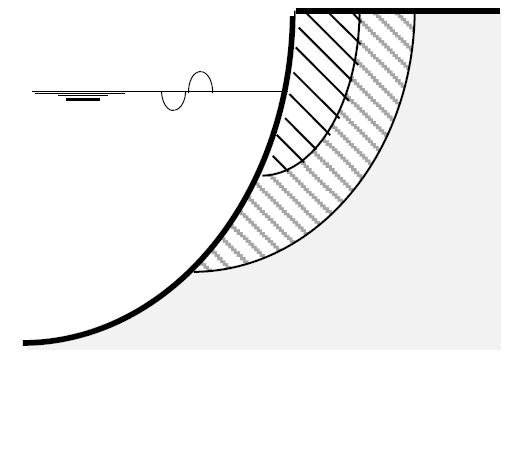
\includegraphics[width=5cm]{figures/Fig4-8a.png} \linebreak
a) vertical layers &
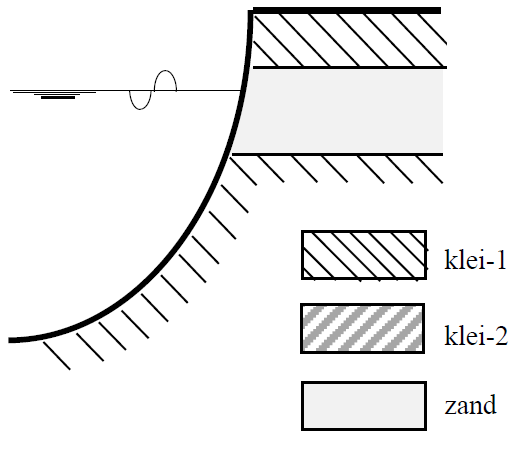
\includegraphics[width=5cm]{figures/Fig4-8b.png} \linebreak
b) horizontal layers \\
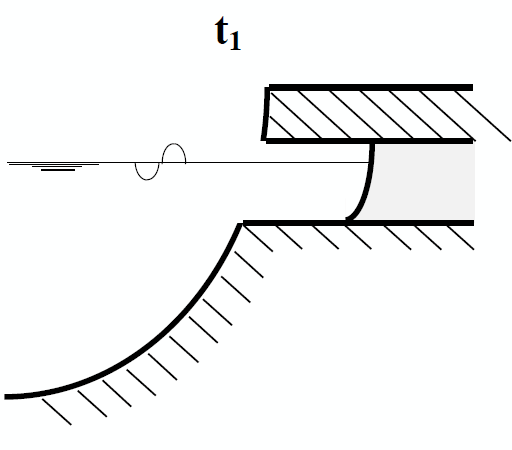
\includegraphics[width=5cm]{figures/Fig4-8c.png} \linebreak
c) erosion process in case of horizontal layers &
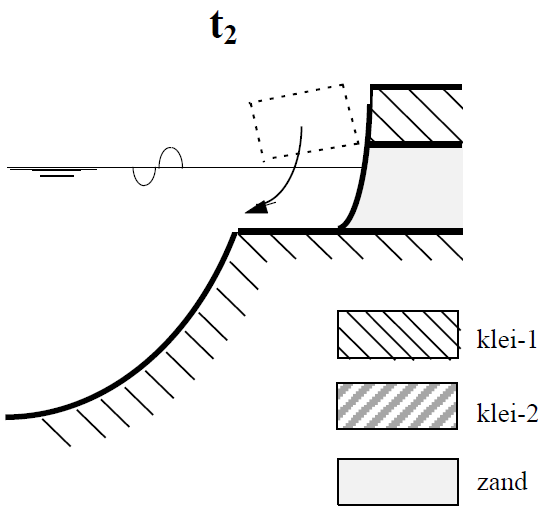
\includegraphics[width=5cm]{figures/Fig4-8d.png} \\
\end{tabular}
\caption{Non-homogeneous banks.}
\label{Fig4.8}
\end{figure}

\subsection{Only erosion along initial bank line}

\dfastbe only estimates the bank erosion along the specified initial bank line (corresponding to the mean discharge).
However, in reality bank erosion may also occur at different heights.

\subsection{Only erosion by ship waves and currents}

\dfastbe only estimates the bank erosion due to the mechanisms of ship waves and currents.
Other bank erosion mechanisms such as wind waves, ground water, freezing or trampling by cattle are currently not included.

\subsection{Profile and bed level remain constant}

The bank erosion affects the local river width and the eroded bank material also results in a bed level change.
This also affects the flow conditions in the river and along the banks in particular.
Since the analysis is based on the results of \dflowfm simulations using the initial geometry, the dynamic feedback via banks and bed levels is not included.
